 
\chapter{OLS with Multiple Covariates}
 \label{chapter::ols-vector}

\section{The OLS formula}

Recall that we have the outcome vector
\[
Y=\left(\begin{array}{c}
y_{1}\\
y_{2}\\
\vdots\\
y_{n}
\end{array}\right)
\]
and covariate matrix
\[
 X=\left(\begin{array}{cccc}
x_{11} & x_{12} & \cdots & x_{1p}\\
x_{21} & x_{22} & \cdots & x_{2p}\\
\vdots & \vdots &  & \vdots\\
x_{n1} & x_{n2} & \cdots & x_{np}
\end{array}\right)=\left(\begin{array}{c}
x_{1}^{\T}\\
x_{2}^{\T}\\
\vdots\\
x_{n}^{\T}
\end{array}\right)
=(X_1,\ldots, X_p)
\]
where $x_{i}^{\T}=(x_{i1},\ldots,x_{ip})$ is the row vector consisting
of the covariates of unit $i$, and $X_j = (x_{1j}, \ldots, x_{nj})^{\T} $ is the column vector of the $j$-th covariate for all units. 


We want to find the best linear fit of the data
$
(x_{i}, \hat{y}_{i} )_{i=1}^{n}
$
with
$$
\hat{y}_{i}=x_{i}^{\T}\hat{\beta} = \hat{\beta}_1 x_{i1} + \cdots + \hat{\beta}_p x_{ip} 
$$
 in the sense that 
\begin{eqnarray*}
\hat{\beta} 
&=&\arg\min_{ b  }n^{-1}\sumn(y_{i}-x_{i}^{\T} b )^{2}\\
&=&\arg\min_{ b }n^{-1}\|Y-X b\|^{2},
\end{eqnarray*}
 where $\hat{\beta}$  is called the OLS coefficient, the $\hat{y}_{i}$'s are called the fitted values, and the $y_i-\hat{y}_{i}$'s are called the residuals. 

The objective function is quadratic in $b$ which diverges to
infinity when $b$ diverges to infinity. So it must have a unique minimizer
$\hat{\beta}$ satisfying the first order condition
\[
-\frac{2}{n}\sumn x_{i}(y_{i}-x_{i}^{\T}\hat{\beta})=0,
\]
which simplifies to 
\begin{equation}
\sumn x_{i}(y_{i}-x_{i}^{\T}\hat{\beta})=0\Longleftrightarrow X^{\T}(Y-X\hat{\beta})=0.\label{eq:normalequation}
\end{equation}
The above equation \eqref{eq:normalequation} is called the {\it Normal equation} of the OLS, which implies the main theorem:
\begin{theorem}
\label{thm:The-OLS-coefficient}The OLS coefficient equals
\begin{eqnarray*}
\hat{\beta}
&=&\left(\sumn x_{i}x_{i}^{\T}\right)^{-1}\left(\sumn x_{i}y_{i}\right) \\
&=& (X^{\T}X)^{-1}X^{\T}Y
\end{eqnarray*}
if $X^{\T}X = \sumn x_{i}x_{i}^{\T}$ is non-degenerate. 
\end{theorem}


The equivalence of the two forms of the OLS coefficient follows from
$$
X^{\T}X = (x_1,\ldots, x_n)  \left(\begin{array}{c}
x_{1}^{\T}\\
x_{2}^{\T}\\
\vdots\\
x_{n}^{\T}
\end{array}\right)
= \sumn x_{i}x_{i}^{\T},
$$
and
$$
X^{\T}Y = (x_1,\ldots, x_n)\left(\begin{array}{c}
y_{1}\\
y_{2}\\
\vdots\\
y_{n}
\end{array}\right)
= \sumn x_{i}y_{i}. 
$$
For different purposes, both forms can be useful. 


The non-degeneracy of $X^{\T}X$ in Theorem \ref{thm:The-OLS-coefficient}  requires that for any non-zero vector $\alpha\in\mathbb{R}^{p},$ we must have
\[
\alpha^{\T}X^{\T}X\alpha=\|X\alpha\|^{2}\neq 0 
\]
which is equivalent to
$$
X\alpha\neq 0,
$$
i.e., the columns of $X$ are {\it linearly independent} \footnote{This book uses different notions of ``independence'' which can be confusing sometimes. In linear algebra, a set of vectors is linearly independent if any nonzero linear combination of them is not zero; see Chapter \ref{chapter::linear-algebra}. In probability theory, two random variables are independent if their joint density factorizes into the product of the marginal distributions; see Chapter \ref{chapter:appendix-rvs}.}. This effectively
rules out redundant columns in the design matrix $X$. If $X_1$ can be represented by other columns $X_1 = c_2 X_2 + \cdots + c_p X_p$ for some $(c_2,\ldots, c_p)$, then $X^{\T} X$ is degenerate. 

Throughout the book, we invoke the following condition unless stated otherwise.
\begin{condition}
The column vectors of $X$ are linearly independent. 
\end{condition}

\section{The geometry of OLS}\label{sec::geometry-ols}


\begin{figure}
\centering
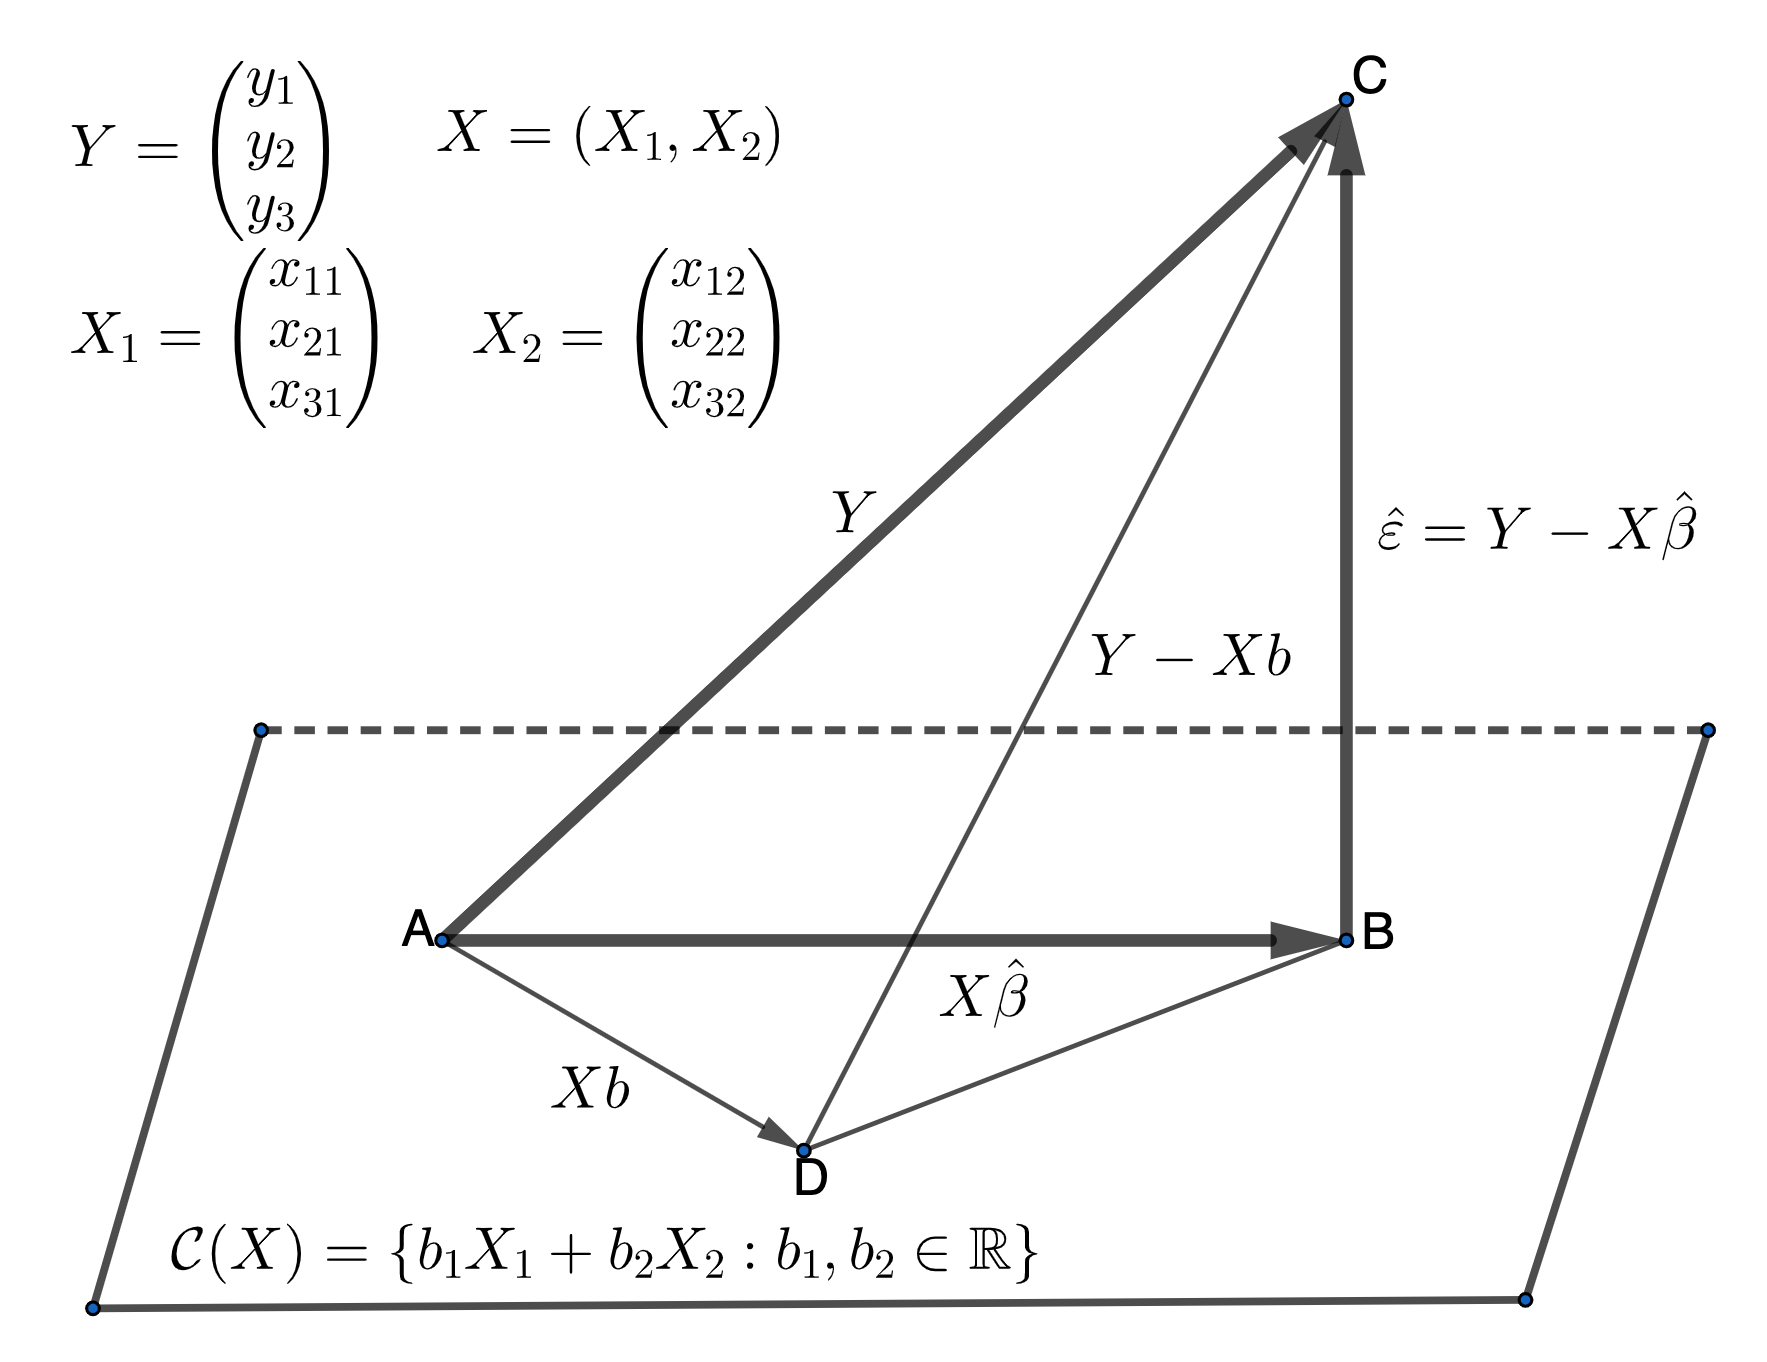
\includegraphics[width = 0.9 \textwidth]{figures/olsgeometry.png}
\caption{The geometry of OLS}\label{fig::olsgeometry}
\end{figure}

The OLS has very clear geometric interpretations. Figure \ref{fig::olsgeometry} illustrate its geometry with $n=3$ and $p=2$. 
For any $b=(b_{1},\ldots,b_{p})^{\T}\in\mathbb{R}^{p}$ and $X=(X_{1},\ldots,X_{p})\in\mathbb{R}^{n\times p}$,
$$
Xb=b_{1}X_{1}+\cdots+b_{p}X_{p}
$$ 
represents a linear combination
of the column vectors of the design matrix $X$. So the OLS problem
is to find the best linear combination of the column vectors of $X$
to approximate the response vector $Y$. Recall that all linear combinations
of the column vectors of $X$ constitute the column space of $X$,
denoted by $\mathcal{C}(X)$ \footnote{Please review Chapter \ref{chapter::linear-algebra} for some basic linear algebra background.}. So the OLS problem is to find the vector
in $\mathcal{C}(X)$ that is the closest to $Y$. Geometrically, the vector
must be the projection of $Y$ onto $\mathcal{C}(X).$ By projection,
the residual vector $\hat{\varepsilon}=Y-X\hat{\beta}$ must be orthogonal
to $\mathcal{C}(X)$, or, equivalently, the residual
vector is orthogonal to $X_{1},\ldots,X_{p}$. This geometric intuition
 implies that
%\begin{align*}
%X_{1}^{\T}\hat{\varepsilon} =0,\ldots,X_{p}^{\T}\hat{\varepsilon}=0  
% \Longleftrightarrow X^{\T} \hat{\varepsilon} =0  
%\end{align*}
\begin{eqnarray*}
&&X_{1}^{\T} \hat{\varepsilon} =0,\ldots,X_{p}^{\T}  \hat{\varepsilon} =0 , \\
&  \Longleftrightarrow &  X^{\T} \hat{\varepsilon}
= \begin{pmatrix}
X_1^{\T} \hat{\varepsilon} \\
\vdots \\
X_p^{\T}\hat{\varepsilon}
\end{pmatrix}
=0,\\
 &  \Longleftrightarrow & X^{\T} (Y-X\hat{\beta}) = 0 ,
\end{eqnarray*}
which is essentially the Normal equation (\ref{eq:normalequation}). 
The above argument gives a geometric derivation of the OLS formula
in Theorem \ref{thm:The-OLS-coefficient}. 



In Figure \ref{fig::olsgeometry}, since the triangle ABC is rectangular, the fitted vector $\hat{Y} = X\hat{\beta}$ is orthogonal to the residual vector $\hat{\varepsilon}$, and moreover, the Pythagorean Theorem implies that
$$
\| Y\|^2 = \| X\hat{\beta} \|^2 + \| \hat{\varepsilon} \|^2.
$$


In most applications,  $X$ contains a column of intercepts $1_{n}=(1,\ldots,1)^{\T}$. In those cases, we have
\[
1_{n}^{\T}\hat{\varepsilon}=0\Longrightarrow n^{-1}\sumn\hat{\varepsilon}_{i}=0,
\]
 so the residuals are automatically centered. 



The following theorem states an algebraic fact that gives an alternative proof of the OLS formula. It is essentially the Pythagorean Theorem for the rectangular
triangle BCD in Figure \ref{fig::olsgeometry}. 

\begin{theorem}\label{thm::geometryofols}
For any $b\in\mathbb{R}^{p},$ we have the following decomposition
\[
\|Y-Xb\|^{2}=\|Y-X\hat{\beta}\|^{2}+\|X(\hat{\beta}-b)\|^{2},
\]
where implies that $\|Y-Xb\|^{2}\geq\|Y-X\hat{\beta}\|^{2}$ with
equality holding if and only if $b=\hat{\beta}.$
\end{theorem}
\begin{myproof}{Theorem}{\ref{thm::geometryofols}}
We have the following decomposition: 
\begin{eqnarray*}
\|Y-Xb\|^{2} 
& =& (Y-Xb)^{\T}(Y-Xb)\\
 & =& (Y-X\hat{\beta}+X\hat{\beta}-Xb)^{\T}(Y-X\hat{\beta}+X\hat{\beta}-Xb)\\
 & =& (Y-X\hat{\beta})^{\T}(Y-X\hat{\beta})+(X\hat{\beta}-Xb)^{\T}(X\hat{\beta}-Xb)\\
 & & +(Y-X\hat{\beta})^{\T}(X\hat{\beta}-Xb)+(X\hat{\beta}-Xb)^{\T}(Y-X\hat{\beta}).
\end{eqnarray*}
The first term equals $\|Y-X\hat{\beta}\|^{2}$ and the second term equals $\|X(\hat{\beta}-b)\|^{2}$. 
We need to show the last two terms are zero. By symmetry of these
two terms, we only need to show that the last term is zero. This is
true by the Normal equation (\ref{eq:normalequation}) of the OLS:
\begin{align*}
(X\hat{\beta}-Xb)^{\T}(Y-X\hat{\beta}) & =(\hat{\beta}-b)^{\T}X^{\T}(Y-X\hat{\beta})=0.\\
\end{align*}
\end{myproof}



 
 


\section{The projection matrix from OLS}

The geometry  in  Section \ref{sec::geometry-ols} also shows that $\hat{Y}=X\hat{\beta}$ is the  solution
to the following problem
\[
\hat{Y}=\arg\min_{v\in\mathcal{C}(X)}\|Y-v\|^{2}.
\]
Using Theorem \ref{thm:The-OLS-coefficient}, we have $\hat{Y}=X\hat{\beta}=HY$, 
where 
\[
H=X(X^{\T}X)^{-1}X^{\T}
\]
is an $n\times n$ matrix. It is called the {\it hat matrix} because it
puts a hat on $Y$ when multiplying $Y$. Algebraically, we can show that
$H$ is a projection matrix because
\begin{eqnarray*}
H^{2} & = & X(X^{\T}X)^{-1}X^{\T}X(X^{\T}X)^{-1}X^{\T} \\
&=& X(X^{\T}X)^{-1}X^{\T} \\
&=& H,
\end{eqnarray*}
and
\begin{eqnarray*}
H^{\T} & = &\left\{ X(X^{\T}X)^{-1}X^{\T}\right\} ^{\T} \\
&=& X(X^{\T}X)^{-1}X^{\T} \\
&=& H.
\end{eqnarray*}
Its rank equals its trace, so 
equals 
\begin{eqnarray*}
\text{rank}(H) = 
\text{trace}(H)&=&\text{trace}\left\{ X(X^{\T}X)^{-1}X^{\T}\right\} \\
&=&\text{trace}\left\{ (X^{\T}X)^{-1}X^{\T}X\right\} \\
&=&\text{trace}(I_{p})=p.
\end{eqnarray*}
The projection matrix $H$ has the following geometric interpretations. 

\begin{proposition}\label{prop::projectionmatrix-geometry}
The projection matrix $H=X(X^{\T}X)^{-1}X^{\T}$ satisfies
\begin{enumerate}
[(G1)]
\item \label{enu:proj1}$Hv=v \Longleftrightarrow  v\in\mathcal{C}(X);$
\item \label{enu:proj2}$Hw=0 \Longleftrightarrow  w\perp\mathcal{C}(X).$
\end{enumerate}
\end{proposition}

Recall that $\mathcal{C}(X)$ is the column space of $X$. 
(G\ref{enu:proj1}) states that projecting any vector in $\mathcal{C}(X)$ onto $\mathcal{C}(X)$ does not change the vector, and (G\ref{enu:proj2}) states that projecting any vector orthogonal to $\mathcal{C}(X)$ onto $\mathcal{C}(X)$ results in a zero vector. 

\begin{myproof}{Proposition}{\ref{prop::projectionmatrix-geometry}}
I first prove (G\ref{enu:proj1}).
If $v\in\mathcal{C}(X),$ then $v=Xb$ for some $b$, which implies
that $Hv=X(X^{\T}X)^{-1}X^{\T}Xb=Xb=v$. Conversely, if $v=Hv$, then $v=X(X^{\T}X)^{-1} X^{\T}v = Xu$ with $u=(X^{\T}X)^{-1} X^{\T}v$, which ensures that $v\in \mathcal{C}(X)$. 

I then prove (G\ref{enu:proj2}). 
If $w\perp\mathcal{C}(X)$, then $w$ is orthogonal to all column
vectors of $X$. So
\begin{eqnarray*}
&&  X_{j}^{\T}w=0\quad(j=1,\ldots,p) \\
&\Longrightarrow & X^{\T}w=0 \\
&\Longrightarrow& Hw=X(X^{\T}X)^{-1}X^{\T}w=0.
\end{eqnarray*}
Conversely, if $Hw=  X(X^{\T}X)^{-1}X^{\T}w =0$, then $w^{\T} X(X^{\T}X)^{-1}X^{\T}w=0$. Because $(X^{\T}X)^{-1}$ is positive definite, we have $X^{\T}w=0$ ensuring that $w\perp\mathcal{C}(X)$. 
\end{myproof}

 

Writing $H=(h_{ij})_{1\leq i,j\leq n}$ and $\hat{y}=(\hat{y}_{1},\ldots,\hat{y}_{n})^{\T}$,
we have another basic identity 
%\begin{eqnarray}\label{eq::ols-fittedvalues}
$$
\hat{y}_{i}=\sum_{j =1}^{n}h_{ij}y_{j} =h_{ii}y_{i}+\sum_{j\neq i}h_{ij}y_{j}.
$$
%\end{eqnarray}
 It shows that the predicted value $\hat{y}_{i}$ is a linear combination
of all the outcomes. Moreover, if $X$ contains a column of intercepts
$1_{n}=(1,\ldots,1)^{\T},$ then 
\[
H1_{n}=1_{n}\Longrightarrow\sum_{j=1}^{n}h_{ij}=1\quad(i=1,\ldots,n),
\]
which implies that $\hat{y}_{i}$ is a weighted average of all the
outcomes. Although the sum of the weights is one, some of them can be negative. 


 
In general, the hat matrix has complex forms, but when the covariates are dummy variables, it has more explicit forms. I give two examples below. 

\begin{example}
\label{eg::treatment-control-H}
In a treatment-control experiment with $m$ treated and $n$ control units, the matrix $X$ contains $1$ and a dummy variable for the treatment:
$$
X = \begin{pmatrix}
1_m& 1_m\\
1_n& 0_n 
\end{pmatrix}.
$$
We can show that 
$$
H = \textup{diag}\{ m^{-1} 1_m 1_m^{\T} , n^{-1} 1_n 1_n^{\T} \}.
$$
\end{example}


\begin{example}
\label{eg::anova-H}
In an experiment with $n_j$ units receiving treatment level $j$ $(j=1,\ldots, J)$, the covariate matrix $X$ contains $J$ dummy variables for the treatment levels:
$$
X =  \textup{diag}\{ 1_{n_1}, \ldots, 1_{n_J} \} .
$$
We can show that 
$$
H = \textup{diag}\{ n_1^{-1} 1_{n_1} 1_{n_1}^{\T} , \ldots, n_J^{-1} 1_{n_J} 1_{n_J}^{\T} \}.
$$
\end{example}


 






\section{Homework problems}

\paragraph{Univariate and multivariate OLS}

Derive the univariate OLS based on the multivariate OLS formula with
$$
X = \begin{pmatrix}
1& x_1 \\
\vdots & \vdots \\
1 & x_n
\end{pmatrix}
$$
where the $x_i$'s are scalars. 


\paragraph{OLS via vector and matrix calculus}

Using vector and matrix calculus, show that the OLS estimator minimizes
$(Y-Xb)^{\T}(Y-Xb)$.


\paragraph{OLS based on pseudo inverse}\label{hw3::ols-pseudoinverse}

Show that $\hat\beta = X^{+} Y$.


Remark: Recall the definition of the pseudo inverse in Chapter \ref{chapter::linear-algebra}. 


\paragraph{Invariance of OLS}\label{hw3::invariance-ols}

Assume that $X^{\T} X$ is non-degenerate and $\Gamma$ is a $p\times p$ non-degenerate matrix. Define $\tilde{X}=X\Gamma$. 
From the OLS fit of $Y$ on $X$, we obtain the coefficient $\hat{\beta}$, the fitted value $\hat{Y}$, and the residual $\hat{\varepsilon}$; from the OLS fit of $Y$ on $\tilde{X}$, we obtain the coefficient $\tilde{\beta}$, the fitted value $\tilde{Y}$, and the residual $\tilde{\varepsilon}$. 

Prove that
$$
\hat{\beta} = \Gamma \tilde{\beta},\quad
\hat{Y} = \tilde{Y},\quad 
\hat{\varepsilon} = \tilde{\varepsilon}. 
$$



Remark: From a linear algebra perspective, $X$ and $X\Gamma$ have the same column space if $\Gamma$ is a non-degenerate matrix:
$$ 
\{   Xb : b\in\mathbb{R}^p \} = \{   X\Gamma c : c\in\mathbb{R}^p \} .
$$
Consequently, there must be a unique projection of $Y$ onto the common column space.  



\paragraph{Invariance of the hat matrix}\label{hw03::invariance-of-H}

Show that $H$ does not change if we change $X$ to $X\Gamma$ where $\Gamma \in \mathbb{R}^{p\times p}$ is a non-degenerate matrix.  


\paragraph{Special hat matrices}\label{hw03::special-H}

Verify the formulas of the hat matrices in Examples \ref{eg::treatment-control-H} and \ref{eg::anova-H}. 




\paragraph{OLS with multiple responses}
\label{hw03::multiple-responses}
 
For each unit $i=1,\ldots, n$, we have multiple responses
$y_i=(y_{i1},\ldots, y_{iq})^{\T}   \in \mathbb{R}^q  $ and multiple covariates $x_i=(x_{i1}, \ldots,x_{ip})^{\T}   \in \mathbb{R}^p $. Define
$$
Y =\begin{pmatrix}
y_{11} &\cdots & y_{1q} \\
\vdots & & \vdots \\
y_{n1} & \cdots & y_{nq}
\end{pmatrix} = \begin{pmatrix}
y_{1}^{\T} \\
\vdots \\
y_{n}^{\T}
\end{pmatrix} 
= (Y_1,\ldots,Y_q) 
\in \mathbb{R}^{n\times q}
$$
and
$$
X = \begin{pmatrix}
x_{11} &\cdots & x_{1p} \\
\vdots & & \vdots \\
x_{n1} & \cdots & x_{np}
\end{pmatrix} = \begin{pmatrix}
x_{1}^{\T} \\
\vdots \\
x_{n}^{\T}
\end{pmatrix} 
= (X_1,\ldots,X_p)
\in \mathbb{R}^{n\times p}
$$
as the response and covariate matrices, respectively. Define the multiple OLS coefficient matrix as
\[ \hat{B} = \arg\min_{B \in \mathbb{R}^{p \times q}}\sum_{i=1}^n \| y_i-B^{\T}x_i \|^2 \]
Show that
$
\hat{B} =(
\hat{B}_1, 
\ldots, 
\hat{B}_q 
)
$
has column vectors 
\begin{eqnarray*}
\hat{B}_1 &=& (X^{\T}  X)^{-1}X^{\T}  Y_1 ,\\
 &\vdots & \\ 
\hat{B}_q &=&(X^{\T}  X)^{-1}X^{\T} Y_q.
\end{eqnarray*}



Remark: 
This result tells us that the OLS fit with a vector outcome reduces to multiple separate OLS fits, or, the OLS fit of a matrix $Y$ on a matrix $X$ reduces to the column-wise OLS fits of $Y$ on $X$. 


\paragraph{Full sample and subsample OLS coefficients}\label{hw3::full-subsample-ols}

Partition the full sample into $K$ subsamples:
$$
X=\left(\begin{array}{c}
X_{(1)}\\
\vdots\\
X_{(K)}
\end{array}\right),\quad 
Y=\left(\begin{array}{c}
Y_{(1)}\\
\vdots\\
Y_{(K)}
\end{array}\right),
$$
where the $k$th sample consists of $(X_{(k)}, Y_{(k)})$ with $X_{(k)} \in \mathbb{R}^{n_k\times p}$ and $ Y_{(k)} \in \mathbb{R}^{n_k} $ being the covariate matrix and outcome vector. Note that $n = \sum_{k=1}^K n_k$ Let $\hat{\beta}$ be the OLS coefficient based on the full sample, and $\hat{\beta}_{(k)}$ be the OLS coefficient based on the $k$th sample. Show that 
$$
\hat{\beta} = \sum_{k=1}^{K}W_{(k)}\hat{\beta}_{(k)},
$$
where the weight matrix equals
$$
W_{(k)} =(X^{\T} X)^{-1} X_{(k)}^{\T}X_{(k)} .
$$

 

\paragraph{Jacobi's theorem}\label{hw03::jacobi}


The set $\{1 ,\ldots, n\}$ has $\binom{n}{p}$ size-$p$ subsets. Each subset $S$ defines a linear equation for $b\in \mathbb{R}^p$: 
$$
Y_S = X_S b   
$$
where $Y_S \in \mathbb{R}^{p}$ is the subvector of $Y$ and $X_S \in \mathbb{R}^{p\times p}$ is the submatrix of $X$, corresponding to the units in $S$. Define the subset coefficient 
$$
\hat{\beta}_S = X_S^{-1} Y_S
$$
if $X_S$ is invertible and  $\hat{\beta}_S =  0 $ otherwise. Show that the OLS coefficient equals a weighted average of these subset coefficients: 
$$
\hat{\beta} = \sum_S   w_S  \hat{\beta}_S
$$
where the summation is over all subsets and 
$$
w_S =  \frac{  |  \det(X_S) | ^2  }{  \sum_{S'}  |  \det(X_{S'}) | ^2 } . 
$$

Remark: To prove this result, we can use Cramer's rule to express the OLS coefficient and use the Cauchy--Binet formula to expand the determinant of $X^{\T} X$. 
This result extends Problem \ref{hw2::pairwise-slope}. 
\citet{berman1988theorem} attributed it to Jacobi. 
\citet{wu1986jackknife} used it in analyzing the statistical properties of OLS. 




